\documentclass[t,aspectratio=169,xcolor=dvipsnames]{beamer}

%\usepackage{soul}
\usepackage{multicol}
\usepackage[utf8]{inputenc}
\usepackage{amsmath}
\usepackage{physics}
\usepackage{siunitx}
\usepackage{graphicx}
\usepackage{multirow}
\usepackage{mathtools}
\usepackage[normalem]{ulem} 

% ----------------------------------------------------------------------------------------------------------------------------------------

\title{
\includegraphics[width=45pt]{oepecsetlogo.png}\\(KTXFI2EBNF) Physics II. Lecture}

\author{Dr.~Gábor FACSKÓ, PhD\\\tiny Assistant Professor / Senior Research Fellow\\\textit{facsko.gabor@uni-obuda.hu}}

\institute{\Tiny Óbuda University, Faculty of Electrical Engineering, 1084 Budapest, Tavaszmező u. 17.\\Wigner Research Centre for Physics, Department of Space Physics and Space Technology, 1121 Budapest, Konkoly-Thege Miklós út 29–33.\\ \url{https://wigner.hu/~facsko.gabor}}

\date{November~24,~2025}

\logo{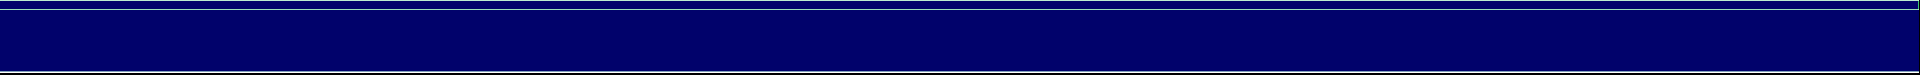
\includegraphics[height=0.9 true cm]{kekcsik.png}}

% ----------------------------------------------------------------------------------------------------------------------------------------

\begin{document}

\frame{\titlepage}

% ----------------------------------------------------------------------------------------------------------------------------------------

\begin{frame}[fragile,squeeze,allowframebreaks]
\frametitle{Common Business}
\begin{itemize}
\setlength{\parskip}{0pt}
\setlength{\itemsep}{0pt}
\item I had time to translate the Hungarian text in the images into English; however, I have not yet had time to upload the updated figures to Moodle. I will do so soon.
\item I have also not yet had time to replace the Hungarian text directly on the images with English labels. I apologize; I will update them shortly.
\item We will not have sufficient time to cover the following topics:
\begin{itemize}
  \item Basic concepts of nuclear physics.
  \item Basic concepts of particle physics.
\end{itemize}
\item I can only briefly outline what these topics include: radioactivity, isotopes, neutron radiation, radiation protection, neutron-induced nuclear fission, thermonuclear fusion, nuclear batteries, types of nuclear reactors, thermonuclear experiments, nuclear weapons, thermonuclear weapons, management of nuclear waste, the Hungarian Nuclear Power Plant in Paks, and future technologies such as advanced reactors, high-temperature reactors, thorium reactors, and modular reactors.

\pagebreak
\item What could I meaningfully tell you about particle physics at this point? For example: hadrons, mesons, leptons, quarks, or particle colliders?
\item We are out of time; therefore, I will send you additional links, or I may record and upload a short personal video exclusively for you.
\item Naturally, none of these topics will be included in the midterm or final examinations.
\end{itemize}
\end{frame}

% ----------------------------------------------------------------------------------------------------------------------------------------

\begin{frame}[fragile,squeeze,allowframebreaks]
\frametitle{Where are we?}
\begin{itemize}
\setlength{\parskip}{0pt}
\setlength{\itemsep}{0pt}
\item \xout{Motion of charged particles in electromagnetic fields.}
  \item \sout{Elements of quantum mechanics. Heisenberg's uncertainty principle. The stationary Schrödinger equation and its applications.}
\item \sout{Limits of the classical conceptual framework. Thermal radiation. Photoelectric effect. Compton effect. The dual nature of electromagnetic radiation. The dual nature of particles.}
\item \sout{Moving reference frames. Inertial forces in accelerating reference frames. Elements of special relativity. Dirac-equation, antimatter.}
\item \sout{The classical theory of atomic structure (Rutherford, Franck-Hertz experiment, Bohr model, quantum numbers, Pauli exclusion principle).}
\item \sout{Physics of condensed matter. Metallic bonding. Electrical conduction in metals based on the free electron model and the wave model. Hall effect. Band theory of solids.}
\pagebreak
\item \sout{Semiconductors. Elements of Fermi-Dirac statistics. Thermoelectric phenomena. Magnetic properties.}
\item \sout{Ferroelectricity. Piezoelectricity and electrostriction. Liquid crystals. Superconductivity.}
\item \textbf{Luminescence. Lasers.} \xout{Basic knowledge of nuclear physics. Basic knowledge of particle physics.}
\end{itemize}
\end{frame}

% ----------------------------------------------------------------------------------------------------------------------------------------

\begin{frame}[fragile,squeeze,allowframebreaks]
\frametitle{Luminescence, Fluorescence, Phosphorescence}
\begin{itemize}
\setlength{\parskip}{0pt}
\setlength{\itemsep}{0pt}
\item Luminescence is the emission of visible light by certain materials when exposed to visible light, X-rays, or radioactive radiation.
\item Unlike thermal radiation, this emission appears even at low temperatures.
\item \underline{Luminescence:} The emission of light in cases where the origin of the emitted radiation is not the temperature of the emitting body is called luminescence. Materials that emit such radiation - i.e., materials that luminesce - are referred to as phosphors.
\item Mechanisms inducing luminescence:
\begin{itemize}
\item Light - photoluminescence.
\item Electrical phenomena - electroluminescence.
\item Radioactive radiation - radioluminescence.
\item Biological processes - bioluminescence (fireflies, certain bacteria).
\end{itemize}
\item Luminescence occurs when a material absorbs incoming radiation and subsequently re-emits it, typically at a different wavelength.

\pagebreak
\item \underline{Duration of luminescence:} The time interval during which a material continues to emit light after the cessation of the excitation is called the luminescence lifetime.
\item Luminescent vs.\ non-luminescent materials:
\begin{itemize}
\item Pure crystals with few defects do \textbf{not} luminesce.
\item Crystal defects are required for luminescence to occur (impurities often enhance the effect).
\item Impurities that facilitate the process are called \textit{activators}.
\item PHOSPHORS = Base material (ZnS, CaS, CdS, KCl, NaCl) + Activator (Ag, Cu, Bi, Mn, Tl)
\end{itemize}

\pagebreak
\item \underline{Fluorescence} is the form of luminescence in which emission ceases almost immediately after the excitation stops (typically $<10^{-6}\,\mathrm{s}$). In short: the light emission effectively ends as soon as the excitation is removed.
\vskip -15 pt
\begin{columns}
  \begin{column}{0.4\textwidth}
  \vskip 10 pt
  \begin{center}
    \includegraphics[width=1.05\textwidth]{images-20251124/page_3_english.png}
  \end{center}
  \end{column}
  \begin{column}{0.65\textwidth}
  \begin{itemize}
  \item An incoming photon elevates an electron of the activator atom from the activator level to the conduction band.
  \item This electron can move freely within the crystal.
  \item If, during its motion, it encounters another activator atom with an available electron site, it recombines — i.e., it returns to the activator level.
  \item The lifetime of the excited state determines the duration of emitted light.
  \end{itemize}
  \end{column}
\end{columns}

\pagebreak
\item \underline{Phosphorescence:} Luminescence in which emission persists for a significantly longer duration — longer than $10^{-5}$–$10^{-4}\,\mathrm{s}$ — is called phosphorescence. In practice, emission may continue for several minutes after excitation ceases.
\item A recombination-inhibiting mechanism must be present. For example, impurities or lattice defects may create “traps’’ within the crystal.
\item These traps can capture electrons wandering through the crystal, preventing recombination with the activator atom.
\item Traps correspond to energetically favorable states immediately below the conduction band.
\item Electrons remain trapped until they receive sufficient energy from lattice vibrations (phonons) to return to the conduction band. They may then become trapped again\dots thus, an electron may undergo multiple trapping cycles.
\item Eventually, upon encountering an activator atom, recombination occurs and luminescent light is emitted.

\pagebreak
\item \underline{Stokes’ theorem:} The frequency of fluorescence light cannot exceed — and its wavelength cannot be shorter than — the frequency or wavelength of the exciting radiation.
\item For the incoming photon:
$$ hf_{0} \ge \Delta W. $$
For the emitted photon:
$$ hf = \Delta W.$$
Thus:
$$ hf_{0} \ge hf \quad \Rightarrow \quad f_{0} \ge f.$$
Using $f = \frac{c}{\lambda}$:
$$ h\frac{c}{\lambda_{0}} \ge h\frac{c}{\lambda},$$
which yields:
$$\frac{1}{\lambda_{0}} \ge \frac{1}{\lambda}.$$
Therefore:
$$\lambda_{0} \le \lambda.$$
\rightline{q.~e.~d.}

\item Applications of phosphorescence:
\begin{itemize}
\item Wavelength conversion: e.g., interior coatings of mercury-vapor lamps or fluorescent tubes.
\item CRT television screens.
\item Oscilloscope screens.
\item Clock dials.
\item etc.\dots
\end{itemize}

\end{itemize}
\end{frame}

% ----------------------------------------------------------------------------------------------------------------------------------------

\begin{frame}[fragile,squeeze,allowframebreaks]
\frametitle{Absorption, Emission, Stimulated Emission, LASER}
\vskip -20 pt
\begin{columns}
\begin{column}{0.3\textwidth}
 \vskip 20 pt
Absorption occurs when atoms absorb energy and transition to higher energy states.
\vskip 40 pt
Spontaneous emission is the natural decay of excited electrons accompanied by photon emission.
\end{column}
\begin{column}{0.7\textwidth}
\begin{center}
\includegraphics[width=0.775\textwidth]{images-20251124/page_8_english.png}
\end{center}
\end{column}
\end{columns}

\pagebreak
\begin{columns}
\begin{column}{0.5\textwidth}
\underline{Population Inversion:} A phenomenon in which more electrons occupy the higher-energy level $W_{2}$ than the lower-energy level $W_{1}$. In this case, the electron population of the higher energy state becomes “more populated’’ than that of the lower energy state. This situation is contrary to the principle of energy minimization. Hence the name: \emph{population inversion}.
\end{column}

\begin{column}{0.5\textwidth}
\vskip -20 pt
\begin{center}
  \includegraphics[width=0.75\textwidth]{images-20251124/page_9_english.png}
\end{center}
\end{column}
\end{columns}

\pagebreak
Induced or stimulated emission  
{\vskip -20 pt}
\begin{center}
\includegraphics[width=0.65\textwidth]{images-20251124/page_10_english.png}
\end{center}
{\vskip -10 pt}
A stimulating external photon can “knock’’ electrons out of the higher energy state, initiating emission. This is why the process is termed \emph{stimulated emission}. The photons produced by stimulated emission are identical in wavelength and are mutually coherent (their phases are the same).
\begin{itemize}
\item \underline{Microwave Amplification by Stimulated Emission of Radiation (MASER):} Devices that amplify microwaves through stimulated emission and subsequently emit microwave radiation are called masers (from the corresponding English acronym).
\item \underline{Light Amplification by Stimulated Emission of Radiation (LASER):} Devices that amplify light through stimulated emission and emit coherent light waves are called lasers (from the English acronym).
\item The first maser was built in 1950; the first laser - a ruby laser - was constructed by Theodore Maiman in 1960.
\item Stimulated emission was predicted by Einstein.

\pagebreak
\item \underline{Laser Energy Scheme:} A genuine two-level laser cannot operate. Pumping excites atoms; spontaneous and stimulated emissions amplify the radiation within a resonator until the light escapes through a partially transmitting mirror.
\begin{center}
\includegraphics[width=0.6\textwidth]{images-20251124/page_12_english.png}
\end{center}

\pagebreak
\item Formation of a Light Avalanche
\vskip -12 pt
\begin{columns}
\begin{column}{0.3\textwidth}
\begin{center}
\includegraphics[width=0.99\textwidth]{images-20251124/page_13.png}
\end{center}
\end{column}
\begin{column}{0.7\textwidth}
\vskip -10 pt
\begin{itemize}
\item The medium initially contains ions or atoms in the ground state.
\item Pumping light (arrows) excites most atoms or ions into higher energy states (empty circles).
\item Excited atoms or ions spontaneously (i.e.\ without external influence) emit photons along the resonator axis (dashed arrows).
\item These photons multiply through stimulated emission and furthermore\dots
\item \dots\,after repeated reflections from the front and back mirrors, the process intensifies in an avalanche-like manner.
\item Once the beam becomes sufficiently strong, it exits the laser tube through the partially transmitting (99\%) mirror $\Rightarrow$ laser.
\end{itemize}
\end{column}
\end{columns}

\pagebreak
\item Laser Examples
\vskip -30 pt
\begin{columns}
\begin{column}{0.3\textwidth}
 \vskip 20 pt
Helium–neon laser  
\vskip 40 pt
Semiconductor lasers.
\end{column}
\begin{column}{0.6\textwidth}
\begin{center}
\includegraphics[width=0.525\textwidth]{images-20251124/page_14_english.png}
\end{center}
\end{column}
\end{columns}

\pagebreak
\item Laser Examples and Applications
\vskip -30 pt
\begin{columns}
\begin{column}{0.4\textwidth}
\vskip 20 pt
\begin{itemize}
\item Ruby laser
\item \underline{Holography:} Invented by Denis Gabor. Interference between the object beam and a reference beam produces a complex interference pattern recorded on film, forming a hologram. The hologram itself \emph{is} the interference pattern.
\end{itemize}
\end{column}
\begin{column}{0.6\textwidth}
\begin{center}
\includegraphics[width=0.525\textwidth]{images-20251124/page_15_1_english.png}\\[6pt]
\includegraphics[width=0.7\textwidth]{images-20251124/page_15_2_english.png}
\end{center}
\end{column}
\end{columns}

\end{itemize}
\end{frame}

% ----------------------------------------------------------------------------------------------------------------------------------------

\begin{frame}
%\frametitle{Minden jó, ha a vége jó}

\vfill
\begin{center}
\textbf{\huge The End}

\bigskip
Thank you for your attention!
\end{center}
\vfill
\end{frame}

\end{document}
